\noindent
Una vez presentados los fundamentos teóricos y las diferentes actividades
para la implementación de cada uno de los métodos, se presentará 
un ejemplo de aplicación. 

Para ello, se propone un \emph{zoom} digital para imágenes panorámicas principalmente
dadas coordenadas de interés. De este modo, en las Figuras \ref{fig:saltillo},
\ref{fig:villahermosa} y \ref{fig:comitan} se presentan fotografías de las 
ciudades de Saltillo, Villahermosa y Comitán respectivamente. Donde para cada caso
se ha propuesto un área de interés de $32x32$ pixeles representada con
un recuadro verde. 

\begin{figure}[H]
    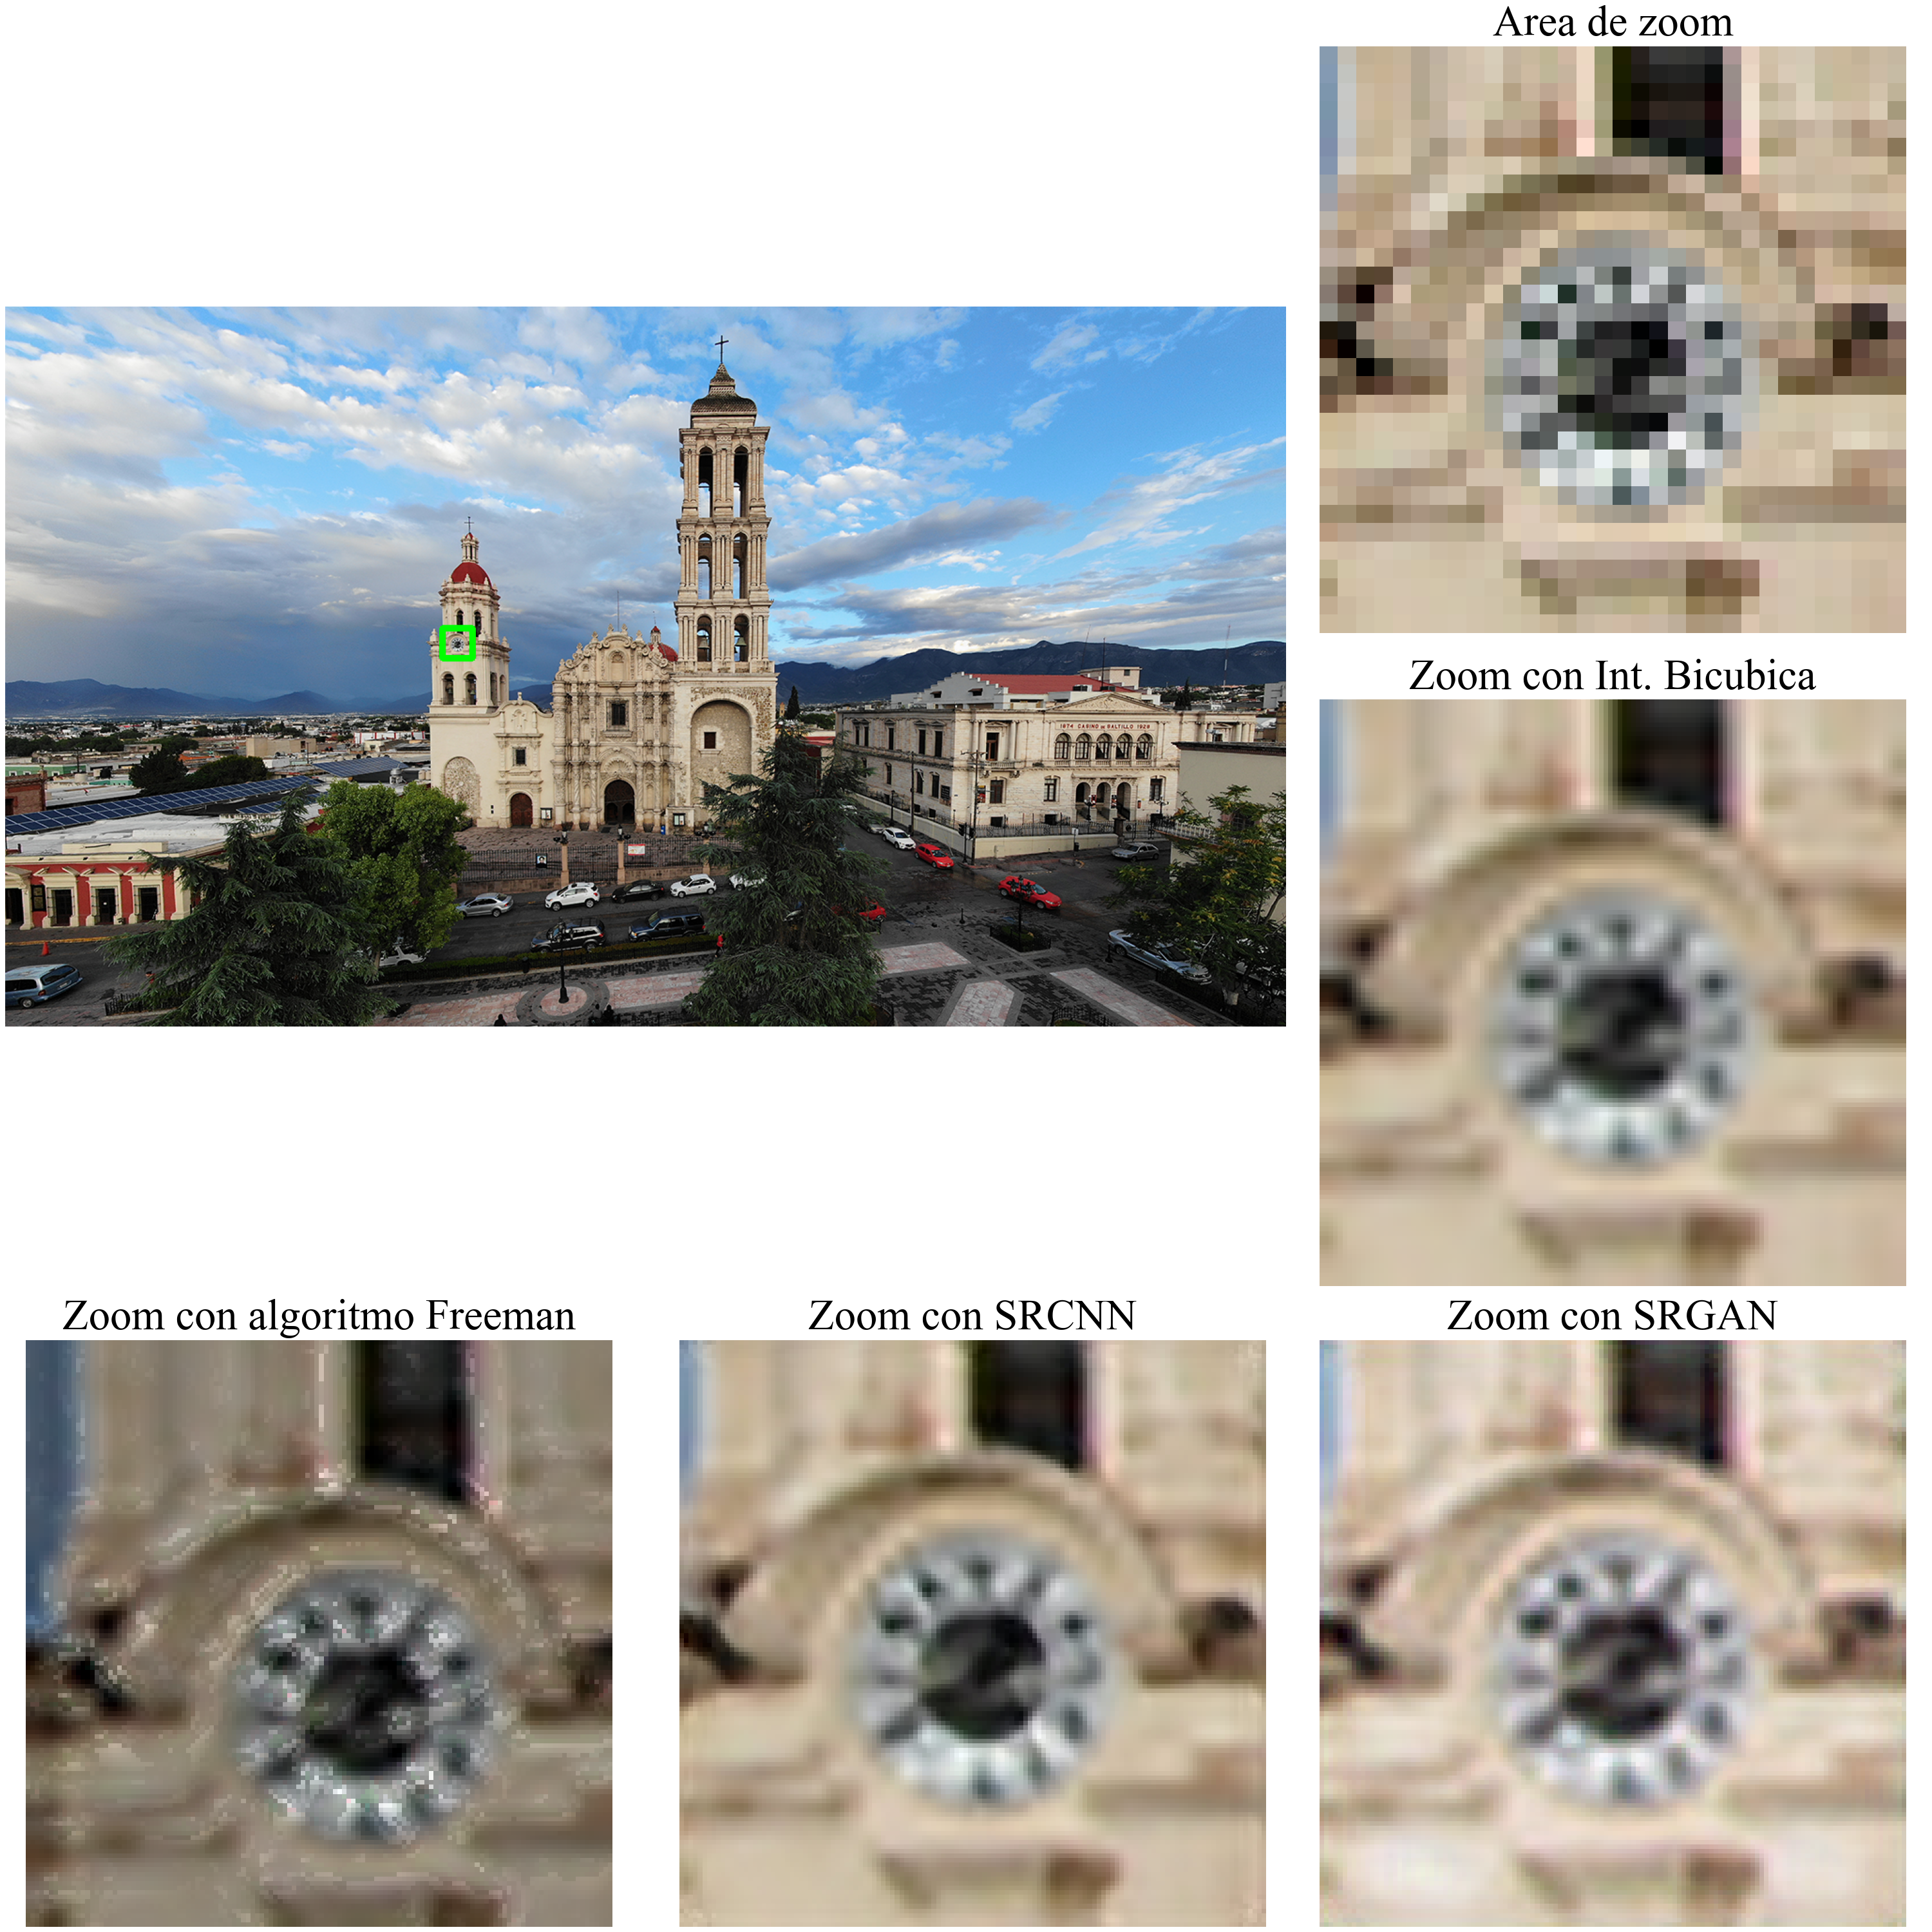
\includegraphics[scale = 0.25]{ ResultadoSaltillo.png}
    \centering
    \caption{Zoom digital en fotografía de Saltillo, Coahuila}
    \label{fig:saltillo}
\end{figure}

Del mismo modo, en cada una de las figuras se encuentra explícitamente
el área de interés o \emph{de zoom}, interpolación bicúbica con el objetivo
de representar y comparar los efectos comentados en la sección de \emph{Antecedentes}.
Así como los tres métodos considerados en este documento para su comparativo.

\begin{figure}[H]
    \includegraphics[scale = 0.25]{ ResultadoVilla.png}
    \centering
    \caption{Zoom digital en fotografía de Villahermosa, Tabasco}
    \label{fig:villahermosa}
\end{figure}

Observe que el comportamiento para cada uno de los métodos es el esperado de
acuerdo a las ventajas y desventajas mencionadas aun cuando el factor de escalado 
es de cuatro veces. 

\begin{figure}[H]
    \includegraphics[scale = 0.25]{ ResultadoComitan.png}
    \centering
    \caption{Zoom digital en fotografía de Comitán, Chiapas}
    \label{fig:comitan}
\end{figure}